\documentclass[12pt]{article}
\usepackage[margin=25mm]{geometry}
\usepackage[T1]{fontenc}
\usepackage[utf8]{inputenc}
\usepackage{amsmath,amssymb,booktabs,array}
\usepackage{graphicx}
\usepackage{setspace,lineno}
\doublespacing
\pagestyle{plain}
\usepackage[colorlinks=true,allcolors=blue]{hyperref}
\newcommand{\gd}{\ensuremath{\gamma\delta}}
\newcommand{\gtd}{\ensuremath{\gamma\!\rightarrow\!\delta}}
\newcommand{\dtg}{\ensuremath{\delta\!\rightarrow\!\gamma}}
\title{Benchmarking single-CDR3 partner recovery in human gamma-delta T-cell receptors under controlled exposure protocols}
\author{Author details pending confirmation}
\date{}
\begin{document}
\linenumbers
\maketitle

\begin{abstract}
\textbf{Background:} Single-chain receptor models can generate plausible CDR3
sequences without recovering the partner recorded for an input chain. A
benchmark must distinguish sequence priors, conditional information, candidate
availability and exposure to related sequences.

\textbf{Methods:} We assembled 9068 unique human gamma-delta T-cell receptor
CDR3 pairs and compared a denoising-pretrained conditional Transformer with
matched constant-source, random-initialization and shuffled-input controls.
The primary endpoint was equal-direction mean query-macro Hit@5 at 64 draws
under component-disjoint splitting. Free generation, fixed-pool retrieval and
additional exposure protocols were evaluated separately, including a separately
trained pair ranker.

\textbf{Results:} Mean target-token negative log likelihood was 1.005 nats for
the pretrained conditional model, 1.013 for the matched constant-source prior
and 1.115 for random initialization. Primary free-generation likelihood Hit@5
was 0.03\%; ranker Hit@5 was 0.06\%, without a reproducible improvement across
fitted comparisons. Recovery was higher under some target-exposed and
source-specific protocols, alongside substantial prior-model recovery.

\textbf{Conclusions:} Denoising pretraining improved target-token likelihood,
while the conditional contribution beyond the matched target prior was modest.
Free recorded-partner recovery remained sparse, and separately trained
reranking did not show reproducible primary benefit. Higher recovery in exposed
populations is sensitive to evaluation design. Biological function and
transfer to distant sequences remain unresolved.
\end{abstract}

\noindent\textbf{Keywords:} gamma-delta T cells; T-cell receptor pairing; CDR3;
sequence generation; evaluation design

\section{Background}
Gamma-delta T-cell receptors (\gd{} TCRs) are heterodimers whose biological interpretation
depends on both chains and the surrounding receptor and cellular context
\cite{gd_review}.
Large sequence collections create opportunities to learn chain-specific
regularities, but abundant unpaired data do not directly reveal which partner
belongs to a given chain. A model that generates plausible target CDR3s may
therefore learn a useful sequence prior without recovering the recorded partner
of a previously unseen input. Distinguishing these behaviors is necessary before
using a score to prioritize receptor candidates.

Public resources now support several related but distinct computational tasks.
UcTCRdb and TCRdb 2.0 include unconventional or gamma/delta repertoires
\cite{uctcrdb,tcrdb2}, while the Observed TCR Space database supports paired-chain
analysis and conditional residue infilling \cite{ots}. TCR-BERT explores
self-supervised TCR representations \cite{tcrbert}. Antigen-specific predictors
and generators such as TCRBinder and TCRdesign address peptide recognition using
paired alpha/beta inputs or antigen-conditioned beta-CDR3 design
\cite{tcrbinder,tcrdesign}; their reported
success does not by itself validate gamma/delta partner-CDR3 generation.
Pretraining loss can also be a poor proxy for downstream benefit
\cite{landry2025}. These distinctions motivate a controlled comparison of
conditional information, target priors and candidate ranking within the same
gamma/delta task.

Related alpha/beta pairing studies have identified inter-chain sequence
constraints \cite{pairing_constraints}. TCRpair predicts functional pairing
within an HLA-A*02:01-restricted alpha/beta setting and includes residues flanking
CDR3 \cite{tcrpair}. These studies motivate testing conditional information, but
their populations, inputs and endpoints differ from gamma/delta partner-CDR3
recovery and their published performance is not a directly transferable baseline.

Here we ask three questions. Does denoising pretraining improve downstream
partner modeling relative to matched random initialization? Does the input
chain improve recorded-partner recovery beyond a matched target prior? Does
separate pairwise ranking improve ordering in fixed and free-candidate settings? We evaluate these questions under explicit exposure
protocols and retain multiple recorded partners per input. The study concerns
the performance of the tested model family on this dataset; it does not seek to
prove that partner prediction is information-theoretically impossible.

The benchmark addresses the lack of a common evaluation that separates target
priors, conditional information, free candidate availability, truth-containing
retrieval and sequence exposure within this gamma-delta task. An exposure
protocol specifies which input chains, target chains and graph components have
been seen during training. Our contribution is a controlled comparison with
saved candidates and explicit endpoint definitions, rather than a claim of
validated receptor function (Figure~\ref{fig:workflow}). Recent epitope-conditioned
diffusion models address a different generation task \cite{dtcr}; a recent
immune-receptor retrieval preprint further motivates checking alignment
baselines and clonal exposure \cite{germline_shortcut}. Neither supplies a direct
performance baseline for single-CDR3 gamma-delta recorded-partner recovery.

\section{Methods}
\subsection{Data assembly and provenance}
The paired corpus contains 9068 unique CDR3 pairs, including 8443 pairs traced
to GSE180059 \cite{gse180059}, 626 to Suo et al.\ through UcTCRdb
\cite{suo2022,uctcrdb}, and one IEDB-export pair with unresolved original-study
provenance \cite{iedb}. Two pairs occur in both major sources. GSE180059 contributes 93.1\% of the
unique-pair union; this source concentration is a defining dataset characteristic.
These are publicly recorded pairings, not a complete biological pairing ground truth.
Extended methods are provided in Additional file 1; dataset composition,
source and split tables are provided in Additional file 2. GSE180059 profiles
fetal and pediatric thymocytes, while the Suo study profiles the developing
prenatal immune system. The paired cohort consequently does not represent the
full adult peripheral gamma/delta repertoire.

Cleaning uppercases and exact-deduplicates canonical amino-acid strings while
retaining source-provided CDR3 boundaries. GEO contigs must satisfy cell,
productive, high-confidence and full-length flags. A library-local barcode is
paired only when exactly one distinct accepted gamma CDR3 and one delta CDR3
remain. Equivalent original cell-quality information is unavailable for some
database exports. Observation-level records retain source membership,
library-local barcodes and available V/J annotations without imputing donor
identity. The models use CDR3 alone. Donor identity cannot be fully recovered from these
exports, so no evaluation is described as donor-independent. Source-provided
CDR3 boundary conventions can differ across collections.

Single-chain inputs total 194887 gamma and 1262692 delta sequences before
pretraining filters. All chains appearing in the paired corpus are excluded
from pretraining, and sequences shorter than six residues are removed. The main
pretraining training pool contains 187092 gamma and 1230589 delta sequences,
with validation sets of 3818 and 25114 sequences. Training and validation are
fully disjoint at the unique CDR3-sequence level. Source experiments
use an additional study-excluded pool containing 186949 gamma and 1230167
delta training sequences, with 3815 and 25106 validation sequences. Both source
protocols use the same filtered pretraining pool. SHA256 manifests identify raw, processed, split and provenance artifacts;
training seeds, selected-checkpoint identifiers and actual exposure appear in Additional file 3.

\subsection{Exposure protocols and validation roles}
We represent unique gamma and delta sequences as the two node sets of a
bipartite graph and recorded pairings as edges. Whole connected components define
three primary train/validation/test splits with seeds 17, 3407 and 2026. Each
split has 7254/907/907 edges and no exact gamma or delta overlap across sets.
The largest component, containing 5005 edges (55.2\%), is assigned wholly to
training (Figure~\ref{fig:data}). Allocation targets edge counts;
it does not optimize source or length balance. Already inspected historical
test memberships are retained unchanged.

Additional unseen-input tasks group by gamma for \gtd{} or delta for \dtg{},
allowing target overlap. Seen-input tasks withhold edges from input chains with
at least three partners while retaining a training edge for each such input.
Strict study holdout removes traceable held-out-study chains from supervised
training, whereas a source-shared diagnostic retains common chains. Both use
the same 626 held-out Suo pairs. Their supervised training sizes differ, so the
contrast is a joint diagnostic of exposure and training composition, not a
causal estimate of memorization. These are study-level exposure sensitivity analyses. They do not provide
donor-independent prospective validation.

Within each original validation set, whole components are assigned to checkpoint
selection, score/sampling tuning and threshold calibration in approximate
50/25/25 proportions with seed 7319. Directional tasks instead preserve source
query groups. Primary split roles contain 453/227/227 edges. No test result
selects a checkpoint, fusion weight, sampling setting or threshold. The primary analysis protocol was specified after earlier exploratory results
had been examined. It is not a preregistration; the earlier estimates, which
used different selection and output-validity rules, are excluded from the
reported primary summaries. Version history is retained in the reproducibility appendix.

The original unseen-gamma validation allocation contained one selection query
with 581 recorded targets and no ranking distractors. Its ranker MRR was
therefore identically one, and generator selection depended on one input. We
retain those results as exploratory diagnostics and repair selection without
changing training, aggregate validation or test membership. Whole gamma-query
groups are reassigned by query count with fixed seed 7319, producing 31/16/16
selection/tuning/calibration queries. Selection now includes 275 edges and at
least 118 eligible distractors per query. Conditional, constant-source and
random-initialized generators and the conditional ranker are refitted for two
seeds. Fixed 64-draw likelihood and ranker results are reported without new
fusion or threshold tuning. This repair is a revision-stage sensitivity analysis.

A separate within-giant-component diagnostic reserves 1000 edges from the
split-17 training graph, removing each edge only while both endpoints retain
training edges. Fixed seeds 1729 and 1730 define reservation and assignment of
500 validation and 500 test edges. The remaining training set contains 6254
edges; every test input and target is still exposed in supervised training.
All 500 validation edges select checkpoints, with no subsequent sampling,
score or threshold tuning. The original primary validation and test edges do
not enter this fit. Because all held edges originate from one component, we
report seed-specific point estimates and event counts without a component-based
inferential interval. This measures withheld-edge recovery within an exposed
component, a distinct population from unseen-component recovery.


\subsection{Generator, pretraining and matched controls}
Figure~\ref{fig:workflow} shows the training and evaluation paths.
The generator is a shared encoder--decoder Transformer with 7396890 parameters,
four encoder and four decoder layers, width 256, eight attention heads,
feedforward width 1024 and dropout 0.1. It tokenizes individual amino acids with
chain identity and control tokens, using a maximum of 64 tokens. The two
conditionals share parameters:
\begin{equation}
p_\theta(d\mid g),\qquad p_\theta(g\mid d).
\end{equation}
Training minimizes teacher-forced target-token negative log likelihood (NLL),
including the end-of-sequence (EOS) token and excluding the chain-control
prediction from the loss.

Denoising uses 20000 steps, batch size 1024, AdamW at learning rate
$3\times10^{-4}$ and 500 warmup steps. Each sequence is masked at 15\% or 30\%
with equal probability. Selected residues are replaced by mask/random/unchanged
tokens at 80/10/10 proportions, followed by short-span deletions targeting
approximately 8\% of positions. Reconstruction is evaluated separately on
corruption-selected residues and against an aligned copy control. The saved
``damaged'' mask includes selected-but-unchanged positions in the 80/10/10 rule
as well as deleted positions; it is not restricted to visibly altered residues.
These teacher-forced
metrics are not free partner-generation accuracy. Raw-frequency, square-root,
balanced, gamma-only and delta-only chain mixtures use the same total number of
sequence draws. Sequence and target-token exposure are reported separately.
The square-root checkpoints are reused from the pair-excluded historical
pretraining, with independently evaluated frozen corruption.

Paired fine-tuning uses at most 1500 steps at batch size 256, learning rate
$2\times10^{-5}$, 200 warmup steps, validation every 100 steps and patience five.
The selection criterion averages known-partner NLL within query, then queries
within direction. Bidirectional models average the two directions equally;
directional exposure diagnostics select using their specified direction only.
Sampling chooses modeled directions equally, input queries uniformly and one
recorded partner uniformly per query.
The constant-source control changes only source residues while retaining
initialization, target sampling and optimization. Random initialization changes only initial weights. It matches downstream
training settings but receives no denoising pretraining, so this is not a
matched-total-computation comparison. Shuffled-input evaluation applies a
deterministic query permutation to the fitted conditional model, disrupting the
input--recorded-partner association. Edge-uniform sampling is a separate control.
The roles of these four controls are summarized in Additional file 1.

The unidirectional sensitivity controls receive at most 750 steps and 100
warmup steps, matching nominal per-direction sequence exposure. Directional
exposure diagnostics instead retain the 1500-step maximum. Actual exposure under early
stopping is recorded. Data-efficiency comparisons use nested complete-component
subsets and both pretrained and random models. The 10/25/50/100\% labels
correspond to 725/1814/2249/7254 edges. The nominal 50\% subset is only 31.0\%
because the 5005-edge component cannot be split. The curve therefore changes
component composition as well as sample size.
All three smaller subsets consist exclusively of singleton components.

\subsection{Separately trained pair ranking and reference methods}
The ranker starts from a separate copy of the selected condition-specific
generator's encoder, after paired fine-tuning. It uses amino-acid-only pooling,
128-dimensional chain-specific projections, a normalized vector dot product
and a two-layer interaction head with hidden width 256 and dropout 0.15 over
the concatenated vectors, their product and absolute difference. The copied encoder and ranking head are optimized on the same training edges
used by the generator. The original generator remains frozen, but the copied
encoder is trainable. Separate training refers to the subsequent parameters
and optimization; neither the representations nor the cohort are independent. Training uses 3000 steps
at batch size 256 and learning rate $3\times10^{-4}$. The first 1500 steps use
multi-positive contrastive loss; the remaining steps use constructed-negative
binary cross-entropy. The primary negative ratio is three per positive, with
half random and half length/terminal-motif matched draws. Ratios one and five
and random-only training provide sensitivity controls. All negative construction
uses training edges only; known training partners are excluded. The best mean
directional selection-validation MRR after explicit-negative training begins
selects the checkpoint.
Positive and constructed-negative classes receive equal BCE loss weight at
every ratio; increasing the ratio changes negative sampling diversity rather
than the total weight of the negative class.

Fixed-pool scorers include conditional likelihood, target-prior likelihood,
deterministically shuffled-input likelihood, their conditional-minus-prior
likelihood difference, ranker, fused score and seeded random scores.
Likelihood scores are negative per-target-token NLL, including EOS; thus the
likelihood difference uses length-normalized log scores rather than the raw
sequence log-probability ratio. Additional
controls are training-target frequency, a shallow length/terminal-feature
logistic model and an exact two-chain edit-neighbor score. For a candidate
$(g,d)$ and training edge set $E_{\rm tr}$, the latter is
\begin{equation}
s_{\rm NN}(g,d)=-\min_{(g',d')\in E_{\rm tr}}
\frac{1}{2}\left[
\frac{\operatorname{Lev}(g,g')}{\max(|g|,|g'|)}+
\frac{\operatorname{Lev}(d,d')}{\max(|d|,|d'|)}\right].
\end{equation}
Every training edge contributes to the minimum. The shallow control is fitted
to training positives and mixed constructed negatives at ratio 1:3, selecting
$C\in\{0.1,1,10\}$ by mean Hit@5 across the four small selection-validation pools.

A complementary nearest-input partner-transfer baseline finds the closest
training input using normalized full-CDR3 Levenshtein distance, resolves ties
lexicographically, and proposes that input's recorded training partners. Targets
are ordered by descending training degree and then lexicographically, retaining
at most 64 unique candidates. A fixed five-neighbor sensitivity concatenates
those lists in neighbor order. No test target is injected into these proposals;
under exact target exclusion their recovery is necessarily zero. For frozen
retrieval pools, a separate nearest-input partner-similarity score ranks each
candidate by its minimum normalized distance to any partner of the single
nearest training input. This similarity extension scores truth-containing
pools and is not direct partner transfer.

\subsection{Free generation, retrieval and calibration}
The primary setting uses 64 draws at temperature one and top-$p=0.95$.
Split-17 primary conditional and constant-source models save 256 draws and
reuse prefixes of 16, 64 and 256. A prespecified six-cell temperature/top-$p$
grid is inspected on split-17 tuning data but does not replace the primary
setting. Validity requires 6--35 canonical residues and an observed EOS token,
allowing 36 decoding steps. Invalid or duplicate draws are not replaced.
Candidates are evaluated both with and without exact training targets. The
exclusion policy may remove legitimate recorded positives in exposed-target
settings, and is reported only as a separate sensitivity analysis. Free
generation does not guarantee that any recorded partner exists among candidates.

For each split and query, fixed candidate pools contain all role-specific
recorded positives and up to 100 unrecorded targets sampled from that split's
target universe using random, length, terminal-motif or edit-neighbor matching.
Full-target retrieval uses the same universe. Other recorded partners are
excluded from distractors without being added as role-specific test positives.
All scorers and model seeds share frozen candidate lists. Unlike free generation,
these retrieval pools include the true targets by construction.
Score ties are resolved by lexicographic target-sequence order. In the primary
chain-disjoint tests, every training-frequency score is zero, so that baseline
is a deterministic tie-order control, not informative frequency prediction.

Direction-specific score means and population standard deviations are estimated
on tuning candidates. A ranker fusion weight from $\{0,.25,.5,.75,1\}$ is shared
across directions and selected by direction-balanced query-macro Hit@5, with
ties favoring less ranker weight. Free and fixed-pool calibration are separate.
An independent calibration subset selects the acceptance threshold by balanced
accuracy against recorded positives and constructed unrecorded combinations;
ties favor the highest threshold, including reject-all. No-positive or
no-negative calibration yields reject-all. Acceptance curves apply fixed
calibration-score quantiles and both endpoints to test data. Pooled AUROC and
AUPRC are reported with positive prevalence, consistent with the limitations of
imbalanced classification summaries \cite{pr_metrics}. These labels and scores
do not define biological specificity or binding probability.

\subsection{Metrics, uncertainty and similarity audit}
For query $q$, let $P_q$ be its recorded test partners, $C_q$ its unique valid
candidates and $C_q^{(K)}$ its first $K$ ranked candidates. Define
\begin{equation}
\mathrm{Coverage}(q)=\mathbf{1}(P_q\cap C_q\ne\varnothing),\qquad
H_K(q)=\mathbf{1}(P_q\cap C_q^{(K)}\ne\varnothing).
\end{equation}
\begin{equation}
R_K(q)=\frac{|P_q\cap C_q^{(K)}|}{|P_q|}.
\end{equation}
If $r_q(t)$ is the one-based candidate rank, reciprocal rank is
$1/\min_{t\in P_q\cap C_q}r_q(t)$ when a partner is present and zero otherwise.
Mean positive rank is $|P_q|^{-1}\sum_{t\in P_q}\widetilde r_q(t)$,
where $\widetilde r_q(t)=r_q(t)$ for present partners and $|C_q|+1$ for absent
partners. MRR averages reciprocal rank across queries. We report query-macro outcomes and positive-count-weighted query
outcomes; the latter yields edge-micro Recall. The primary endpoint is the
equal-direction mean of query-macro Hit@5 at 64 draws, reported separately for
likelihood, ranker and fused ordering. Per-fit event counts and query-level results appear in Additional file 4;
all frozen retrieval pools, candidate hashes and split assignments are supplied
in Additional file 5. NLL, token-weighted NLL, raw ordering,
validity, uniqueness, novelty and diversity are secondary summaries.

We use 2000 paired cluster-bootstrap replicates over complete test components,
or source-query groups for directional tasks. Joint directional endpoints use
the same component resample but average direction-specific query means equally.
Model comparisons align query identities, positives and cluster labels; fixed
pools must also have identical hashes. Two model seeds are averaged within each
split before descriptive mean and standard deviation across three splits.
Repeated splits and seeds are not independent biological subjects. Intervals
condition on fitted models and saved candidates, and are descriptive without
family-wise multiplicity adjustment. Zero-event percentile intervals of $[0,0]$
are not population upper bounds; an explicitly labeled iid Wilson reference is
provided for binary query events only, not fractional Recall.

Every paired chain is compared with supervised and pretraining references using
raw and length-normalized Levenshtein distances on complete CDR3, internal
residues (excluding three residues at each end) and terminal residues. Exact
minimum witnesses are saved. Full-sequence strata are 0, 1, 2 and at least 3.
The distant subset requires both source and eligible recorded target to be at
distance at least three from both reference pools. Edge-defined strata retain
the original candidate lists and test-cluster identities. Empty and single-cluster
strata are explicit. Source, length, number of partners and training-target
overlap are additional descriptive strata.

\subsection{Computational provenance and AI assistance}
The computational environment uses Python 3.10.20 and PyTorch 2.7.1 with CUDA
12.6. The original benchmark uses A800 GPUs; revision diagnostics use RTX 3090
GPUs with the frozen scientific settings. No hardware-performance
comparison is inferred. Training and evaluation devices, commands, seeds and numeric
settings are recorded per run. Frozen code and input/output hashes link fitted
checkpoints, saved candidates and statistical analyses. Hardware timings are
descriptive rather than a controlled device benchmark.

An OpenAI coding assistant was used for code development, experimental
orchestration, artifact checking, literature organization and manuscript drafting.
The analysis files preserve the computational workflow. Scientific interpretation and responsibility remain with the human authors.
Source, environment, configuration and execution records are provided in
Additional file 6.

\section{Results}
\subsection{The paired corpus is highly concentrated and near-neighbor exposed}
The 9068 pairs involve 3944 gamma and 6989 delta CDR3s. There are 3294 graph
components, of which 2897 contain one edge. The largest component contains
5005 edges (55.2\% of the corpus) and remains wholly in training. The maximum
recorded gamma and delta degrees are 581 and 140, respectively; 767 gamma and
519 delta nodes have more than one partner. A unique CDR3 therefore does not
have a unique label in this dataset. GSE180059 contributes 93.1\% of pairs,
limiting the effective diversity of the paired supervision
(Table~\ref{tab:data}; Figure~\ref{fig:data}).

% BEGIN GENERATED TABLE data_table.tex
\begin{table}[ht]
\centering
\caption{Primary split structure and proximity to the pretraining pool. Distance bins use unique test gamma queries; these are not donor-level external tests. Distant edges require both chains to be at least three edits from supervised and pretraining references.}
\label{tab:data}
\small
\setlength{\tabcolsep}{3pt}
\begin{tabular}{p{0.4200\linewidth}p{0.1600\linewidth}p{0.1600\linewidth}p{0.1600\linewidth}}
\toprule
Split seed & 17 & 3407 & 2026\\
\midrule
Training/validation/test edges & 7254/907/907 & 7254/907/907 & 7254/907/907\\
Test gamma queries & 529 & 523 & 525\\
Test delta queries & 900 & 906 & 904\\
Gamma queries one edit from pretraining & 487 & 494 & 493\\
Gamma queries at least three edits from pretraining & 8 & 7 & 4\\
Distant test edges & 5 & 5 & 3\\
Largest-component assignment & Training & Training & Training\\
\bottomrule
\end{tabular}
\end{table}
% END GENERATED TABLE data_table.tex

\subsection{Exact-chain exclusion leaves extensive near-neighbor exposure}
All primary cross-partition exact-chain intersections are empty. Nevertheless,
487/529, 494/523 and 493/525 test gamma queries are one edit from a pretraining
sequence. Requiring distance at least three on both chains and against both
reference pools leaves 5, 5 and 3 primary-test edges. Neither source test has any
edge satisfying this condition. Consequently, a positive overall result under
exact-chain exclusion would not establish robust distant-sequence generalization.

\subsection{Denoising pretraining improves single-chain reconstruction}
On the frozen square-root-pretrained validation corruptions, selected-residue
accuracy is 71.3\% and 70.3\% for gamma and 64.1\% and 64.7\% for delta across
the two seeds. Corresponding aligned-copy accuracy is 6.9\%/6.3\% for gamma and
6.7\%/6.2\% for delta. This shows reconstruction beyond the specified aligned-copy sanity control. It does not establish that pretraining improves recorded partner
recovery; that question requires the downstream matched comparisons.

\subsection{Pretraining improves likelihood with a modest conditional contribution}
Across the three primary splits, the pretrained conditional model has an
equal-direction query-macro NLL of $1.005\pm0.004$ nats per target token,
compared with $1.013\pm0.003$ for the matched constant-source model,
$1.115\pm0.006$ for random initialization and $1.018\pm0.003$ with shuffled
inputs (Table~\ref{tab:primary}; Figure~\ref{fig:primary}). Here and below,
the three split means each average two model seeds, and the reported standard
deviation describes variation between splits. All six fitted contrasts of conditional minus constant-source NLL are negative, ranging from approximately $-0.009$ to
$-0.006$, with paired component-bootstrap intervals below zero. The analogous
conditional-minus-random contrasts range from $-0.115$ to $-0.104$
(Table~\ref{tab:paired}). These differences support a modest conditional
likelihood contribution under the specified training protocol.

\subsection{Free recorded-partner recovery remains sparse}
Likelihood improvement did not translate into reliable free recorded-partner
recovery. The primary endpoint is much smaller. At 64 draws with
training targets allowed, conditional coverage averages $0.88\pm0.19\%$ and
likelihood Hit@5 $0.03\pm0.03\%$. The constant-source model has
$0.50\pm0.10\%$ coverage and no top-five hits; random initialization has
$0.68\pm0.11\%$ coverage and no likelihood top-five hits. Conditional coverage
is strongly directional: $0.09\pm0.16\%$ for \gtd{} versus
$1.66\pm0.23\%$ for \dtg{}. There are no \gtd{} top-five hits in any primary
conditional fit. For \dtg{}, likelihood recovers two of 900 queries for
split 17/model seed 3407 and one of 906 for split 3407/model seed 3508;
the other four fits have zero events. These overlapping splits and repeated
fits are not pooled as independent biological observations.

Separately trained reranking yields equal-direction Hit@5 of $0.06\pm0.03\%$, with
all six paired ranker-minus-likelihood intervals including zero. Free-candidate
tuning selects zero ranker weight in every primary fit, so fused ordering has
the same primary Hit@5 as likelihood. The matched contrasts therefore provide
clearer evidence for improved likelihood than for a reproducible improvement
in the prespecified free-recovery endpoint. Candidate scarcity is a central failure mode: a ranker cannot recover a
recorded partner absent from the candidate set. Additional file 4 retains
coverage, likelihood, ranker and fused event counts for every fit. A zero-event
bootstrap interval does not establish absence of possible recovery in the population.

% BEGIN GENERATED TABLE primary_table.tex
\begin{table}[ht]
\centering
\caption{Free generation at 64 draws with training targets allowed. Values are means and descriptive standard deviations of three split means, each averaging two model seeds. NLL is in nats per target token; coverage and Hit@5 are percentages. The equal mean weights directions equally. A dash denotes an unavailable scorer, not a zero outcome.}
\label{tab:primary}
\small
\setlength{\tabcolsep}{3pt}
\begin{tabular}{p{0.2200\linewidth}p{0.1360\linewidth}p{0.1360\linewidth}p{0.1360\linewidth}p{0.1360\linewidth}p{0.1360\linewidth}}
\toprule
Model / direction & NLL & Coverage & Likelihood Hit@5 & Ranker Hit@5 & Fused Hit@5\\
\midrule
Conditional / \gtd{} & 1.253 $\pm$ 0.008 & 0.09 $\pm$ 0.16 & 0.00 $\pm$ 0.00 & 0.00 $\pm$ 0.00 & 0.00 $\pm$ 0.00\\
Conditional / \dtg{} & 0.757 $\pm$ 0.003 & 1.66 $\pm$ 0.23 & 0.06 $\pm$ 0.06 & 0.11 $\pm$ 0.06 & 0.06 $\pm$ 0.06\\
Conditional / Equal mean & 1.005 $\pm$ 0.004 & 0.88 $\pm$ 0.19 & 0.03 $\pm$ 0.03 & 0.06 $\pm$ 0.03 & 0.03 $\pm$ 0.03\\
Constant source / \gtd{} & 1.257 $\pm$ 0.007 & 0.00 $\pm$ 0.00 & 0.00 $\pm$ 0.00 & -- & --\\
Constant source / \dtg{} & 0.769 $\pm$ 0.003 & 1.00 $\pm$ 0.20 & 0.00 $\pm$ 0.00 & -- & --\\
Constant source / Equal mean & 1.013 $\pm$ 0.003 & 0.50 $\pm$ 0.10 & 0.00 $\pm$ 0.00 & -- & --\\
Random init. / \gtd{} & 1.377 $\pm$ 0.010 & 0.03 $\pm$ 0.05 & 0.00 $\pm$ 0.00 & 0.00 $\pm$ 0.00 & 0.00 $\pm$ 0.00\\
Random init. / \dtg{} & 0.853 $\pm$ 0.005 & 1.33 $\pm$ 0.22 & 0.00 $\pm$ 0.00 & 0.07 $\pm$ 0.03 & 0.02 $\pm$ 0.03\\
Random init. / Equal mean & 1.115 $\pm$ 0.006 & 0.68 $\pm$ 0.11 & 0.00 $\pm$ 0.00 & 0.04 $\pm$ 0.02 & 0.01 $\pm$ 0.02\\
Shuffled input / \gtd{} & 1.267 $\pm$ 0.006 & 0.03 $\pm$ 0.05 & 0.00 $\pm$ 0.00 & 0.00 $\pm$ 0.00 & 0.00 $\pm$ 0.00\\
Shuffled input / \dtg{} & 0.769 $\pm$ 0.001 & 1.33 $\pm$ 0.10 & 0.02 $\pm$ 0.03 & 0.15 $\pm$ 0.08 & 0.04 $\pm$ 0.03\\
Shuffled input / Equal mean & 1.018 $\pm$ 0.003 & 0.68 $\pm$ 0.07 & 0.01 $\pm$ 0.02 & 0.07 $\pm$ 0.04 & 0.02 $\pm$ 0.02\\
\bottomrule
\end{tabular}
\end{table}
% END GENERATED TABLE primary_table.tex

% BEGIN GENERATED TABLE paired_primary_table.tex
\begin{table}[ht]
\centering
\caption{Primary paired contrasts. The 95\% component-bootstrap percentile intervals condition on each fitted model pair and its saved samples. All endpoints are equal-direction query means at 64 draws. C denotes the pretrained conditional model and P the matched constant-source prior. NLL differences are nats per token; Hit@5 differences are percentage points. Negative NLL and positive Hit@5 differences favor the first named condition. Ranker and fusion contrasts reorder the conditional model's identical candidates. Intervals are not adjusted for multiple comparisons; a zero-event [0,0] interval is not a population upper bound.}
\label{tab:paired}
\small
\setlength{\tabcolsep}{3pt}
\begin{tabular}{p{0.2200\linewidth}p{0.1360\linewidth}p{0.1360\linewidth}p{0.1360\linewidth}p{0.1360\linewidth}p{0.1360\linewidth}}
\toprule
Split / model seed & NLL: C minus P & Hit@5: C minus P & NLL: C minus random & Hit@5: ranker minus likelihood & Hit@5: fused minus likelihood\\
\midrule
17 / 3407 & -0.007 [-0.010, -0.004] & 0.11 [0.00, 0.27] & -0.109 [-0.116, -0.102] & 0.00 [-0.21, 0.22] & 0.00 [0.00, 0.00]\\
17 / 3508 & -0.009 [-0.012, -0.006] & 0.00 [0.00, 0.00] & -0.104 [-0.111, -0.097] & 0.00 [0.00, 0.00] & 0.00 [0.00, 0.00]\\
3407 / 3407 & -0.006 [-0.009, -0.004] & 0.00 [0.00, 0.00] & -0.115 [-0.123, -0.108] & 0.00 [0.00, 0.00] & 0.00 [0.00, 0.00]\\
3407 / 3508 & -0.006 [-0.009, -0.004] & 0.06 [0.00, 0.17] & -0.111 [-0.118, -0.104] & 0.00 [-0.17, 0.16] & 0.00 [0.00, 0.00]\\
2026 / 3407 & -0.009 [-0.011, -0.006] & 0.00 [0.00, 0.00] & -0.114 [-0.121, -0.106] & 0.06 [0.00, 0.17] & 0.00 [0.00, 0.00]\\
2026 / 3508 & -0.008 [-0.010, -0.005] & 0.00 [0.00, 0.00] & -0.106 [-0.113, -0.099] & 0.11 [0.00, 0.28] & 0.00 [0.00, 0.00]\\
\bottomrule
\end{tabular}
\end{table}
% END GENERATED TABLE paired_primary_table.tex

\subsection{Retrieval depends on direction and distractor construction}
Fixed-pool retrieval is substantially easier than free generation because each
pool includes the recorded targets (Figure~\ref{fig:retrieval}). In random
small pools, mean conditional-likelihood Hit@5 is 8.9\% for \gtd{} and
13.5\% for \dtg{}, compared with 8.5\% and 11.5\% for the target prior and
8.0\% and 5.1\% for seeded random scores. In full-target retrieval,
conditional likelihood reaches 1.2\% and 4.2\%, compared with 1.1\% and
3.8\% for the prior. These are descriptive averages; the query-level reports
retain paired intervals and pool membership for each fitted comparison.

The conditional-minus-prior score is particularly sensitive to direction.
For \gtd{}, it raises motif-pool Hit@5 from 5.4\% for conditional likelihood
to 12.4\%, but a shallow length/terminal-feature model already reaches 11.8\%.
For \dtg{}, the same difference score gives 6.0\% in motif pools and 1.0\%
in full retrieval, below conditional likelihood's 8.0\% and 4.2\%.
The separately trained ranker gives 8.3\%/5.1\% in motif pools and 1.1\%/1.4\%
in full retrieval for the two directions. No single scorer dominates across
these evaluation conditions. In particular, gains within truth-containing
pools do not establish that a free sampler supplies the recorded partner.

The nearest-input partner-similarity control reaches mean random-pool Hit@5
of 9.2\% for \gtd{} and 7.9\% for \dtg{}, and full-pool Hit@5 of 1.5\% in
both directions. It is competitive with conditional likelihood in some
\gtd{} pools but does not dominate the \dtg{} comparison. Direct transfer
of training partners from either one or five nearest inputs has zero primary
hits, as expected from complete supervised-target exclusion. Its proposals
contain at most 64 unique training targets, rather than 64 stochastic draws.
These two baseline endpoints are kept separate in Additional file 4.

\subsection{Pretraining improves likelihood across nested graph subsets, but recovery remains sparse}
Pretraining gives lower NLL than random initialization at every actual training
size (Figure~\ref{fig:efficiency}). At 725 edges, two-seed mean pretrained NLL
is 1.273/0.780 for \gtd{}/\dtg{}, compared with 1.392/0.849 for random
initialization. At 2249 edges the corresponding values are 1.255/0.771 and
1.375/0.838. Moving to 7254 edges changes them to 1.256/0.754 and
1.376/0.847. The random model's \dtg{} NLL does not improve monotonically
with more edges, and pretrained \gtd{} NLL largely plateaus beyond 1814.

The NLL advantage does not translate into a consistent small-data recovery
advantage. Pretrained \dtg{} likelihood Hit@5 across 725/1814/2249/7254
edges is 0.06/0.17/0.33/0.11\%, while the random model gives
0.22/0.44/0.17/0.00\%. Every \gtd{} likelihood Hit@5 remains zero. These
tiny event rates, two-seed variation and the addition of the giant component
only at full data prevent interpreting this curve as a pure sample-complexity
estimate. It is a sensitivity analysis of the specified nested graph subsets.

\subsection{Negative-sampling sensitivity does not resolve candidate scarcity}
Alternative negative ratios and matching policies show no reproducible
free-recovery gain over the primary ranker. All paired intervals include zero;
no ranker supplies sequences absent from the saved free candidate set. Detailed
negative-sampling, pretraining-mixture and directional-budget sensitivities are
reported in Additional file 1.

% BEGIN REVISION DIAGNOSTIC RESULTS
\subsection{Repaired unseen-gamma selection does not establish a conditional recovery advantage}
The revised validation has 31 selection queries with eligible distractors, and
ranker selection MRR is no longer identically one: the selected values are
0.1405 and 0.1618. Training and test memberships remain unchanged. At 64 free
draws, conditional likelihood recovers 8/64 and 10/64 queries, compared with
8/64 and 9/64 for constant source, 10/64 and 8/64 for random initialization,
and 6/64 and 7/64 for shuffled input. These counts also equal coverage for
each fitted generator. Conditional-minus-prior Hit@5 differences are 0.00
percentage points (95\% source-query interval $[0.00,0.00]$) and 1.56 points
($[0.00,4.69]$). The small number of discordant events limits inference.
Ranker ordering recovers 6/64 and 8/64 queries, two fewer than likelihood in
each seed. One-neighbor and five-neighbor direct partner transfer recover 3/64
and 7/64 queries, respectively. The repaired test still permits target
exposure: 252 distinct recorded target deltas also occur in training.
These revision results supersede the original single-query-selection
diagnostic, whose estimates remain in Additional file 1. They do not establish
a reproducible conditional free-recovery advantage over the matched prior.

\subsection{Withheld edges within the giant component have high prior and shuffled recovery}
Within the exposed giant component, conditional coverage is 70/177 and 62/177
gamma queries and 155/261 and 164/261 delta queries. Likelihood Hit@5 is
60/177 and 50/177 for \gtd{} (33.90\%/28.25\%), and 123/261 and 118/261 for
\dtg{} (47.13\%/45.21\%; Figure~\ref{fig:protocols}). Constant-source
Hit@5 is 47/177 in both gamma-query fits and 113/261 and 121/261 for delta
queries. Shuffled-input counts are 57/177 and 54/177, and 126/261 and 116/261,
respectively. Random initialization yields 32/177 and 27/177, and 121/261 and
124/261. Thus, much of the high recovery persists without the correct input
association; a conditional-minus-prior advantage is not consistent across
directions and seeds.

Ranker ordering gives 30/177 and 35/177 gamma-query hits and 71/261 and 94/261
delta-query hits, below likelihood in all four fits. Direct transfer from one
nearest input has zero hits in both directions: the nearest input is the query
itself, whose remaining training partners exclude its withheld edges. The fixed five-neighbor
sensitivity recovers 4/177 and 57/261 queries. These proposals contain copied
training partners and use a different candidate mechanism from stochastic
generation. All 500 test edges retain both endpoints in supervised training
and originate from one original graph component. The results are point
estimates and counts, without an inferential component-bootstrap interval.
Their contrast with the primary task describes different graph populations
and training composition, rather than distant or unseen-component transfer.
% END REVISION DIAGNOSTIC RESULTS

\subsection{Directional diagnostics allow recovery of exposed targets}
Other directional tasks also have higher recovery than the both-chain-unseen
primary task (Figure~\ref{fig:protocols}). For unseen delta inputs, conditional \dtg{} Hit@5 is 39.75\%/38.51\%,
compared with 41.61\%/39.13\% for the prior. This test has 161 queries and
244 distinct recorded target gammas shared with training. Thus, substantial
recovery in a target-exposed task does not itself demonstrate an input-specific
advantage. In seen-input/unseen-edge tests, conditional Hit@5 is
6.89\%/6.67\% for \gtd{} versus 5.33\%/5.33\% for the prior, and
32.58\%/34.09\% for \dtg{} versus 30.30\%/29.92\%. These populations,
edge counts and permissible overlaps differ from the primary test and are
reported as distinct diagnostics, with source-query-group intervals.
For seen delta inputs, conditional-minus-prior Hit@5 differences are 2.27
percentage points (95\% interval $[-1.52,6.06]$) and 4.17 points
($[0.38,8.33]$). The latter fitted contrast is positive, but the two-seed
result is not uniform and does not transfer to both-chain-unseen generation.

\subsection{Study-level exposure sensitivity is directional and component-concentrated}
Strict study holdout has 207 gamma and 419 delta queries over 626 pairs.
Conditional \dtg{} likelihood Hit@5 is 11.93\%/10.26\%, compared with
6.68\%/6.44\% for constant source and 8.83\%/9.79\% for shuffled input.
Conditional-minus-prior differences are 5.25 percentage points with a 95\%
component interval $[0.00,6.23]$ and 3.82 points with $[0.00,4.48]$;
both intervals reach zero despite positive fitted differences.
When shared supervised chains are retained, the corresponding conditional
values increase to 47.49\%/44.39\%; constant source already reaches
43.68\%/43.20\%, and shuffled input reaches 43.68\%/43.91\%.
The shared-source conditional-minus-prior differences are 3.82 percentage
points ($[-2.13,4.69]$) and 1.19 points ($[0.00,1.42]$), again with paired
component intervals including zero.
For \gtd{}, conditional likelihood Hit@5 is zero in both seeds under both
source protocols. Source results therefore cannot be reduced to uniform
failure, nor can high \dtg{} recovery be attributed entirely to conditioning.

The source test contains 90 components, with 529 of 626 edges and 323 of 419
delta queries in its largest component. A post-hoc description of the saved
query outcomes finds 50 of 50 and 42 of 43 strict-source conditional top-five
hits in that component. The corresponding shared-source counts are 198 of 199
and 184 of 186. This concentration motivates the clustered uncertainty rather
than treating all hits as independent replications. The source protocols share
the same test set and filtered pretraining pool, but supervised training contains
4956 versus 7597 edges. Shared-source training overlaps the test in 144 gamma
and 13 delta sequences. Exposure and training composition therefore change
together. Neither protocol supports a donor-independent or distant-sequence
generalization claim.

Ranker-only \dtg{} Hit@5 is 3.10\%/2.86\% under strict source holdout and
14.32\%/13.60\% under shared source, below likelihood in all four fits.
The higher source-task recovery consequently does not rescue the proposed
separate-ranking benefit.

\subsection{More sampling increases coverage without ensuring top-five recovery}
Split-17 conditional \dtg{} coverage increases from 0.67\%/0.33\% at 16
draws to 2.33\%/1.44\% at 64 and 6.33\%/6.22\% at 256 for model seeds
3407/3508. Nevertheless, with training targets allowed, likelihood Hit@5 is
0.22\%/0.11\%, 0.22\%/0.00\% and 0.00\%/0.00\%, respectively
(Figure~\ref{fig:budget}). Additional samples can introduce high-scoring
competitors as well as recorded partners. The 256 draws average approximately
203 unique valid gamma candidates per query, but only about 53\% of raw
gamma draws differ from supervised-training targets. For \gtd{}, approximately
88\% of draws are novel and about 244 unique candidates remain at 256 draws;
coverage is 0.57\% in each seed and likelihood Hit@5 remains zero.

Excluding exact training targets changes ordering without increasing the
sampling budget. Because primary-test targets are chain-disjoint from training,
their coverage is unchanged. At 256 draws, \dtg{} likelihood Hit@5 increases
to 1.89\%/2.44\%, while \gtd{} reaches 0.57\%/0.19\%. This policy result
is reported separately from the frozen primary endpoint. It cannot be applied
unchanged as a general advantage in shared-target tasks, where exclusion may
remove a legitimate test partner.

The six-cell tuning-only temperature/top-$p$ grid has zero likelihood Hit@5
in both directions for both fitted seeds at 64 draws. The prespecified tie
rule retains temperature one and top-$p=0.95$; these sparse tuning outcomes
do not establish an improved decoding setting. All grid cells and their
coverage, validity, uniqueness and novelty are included in the supplement.

Free-candidate calibration contains no recorded \gtd{} positive in any
primary fit, triggering the specified reject-all rule. The \dtg{} calibration
sets contain only one to six recorded positive candidates. Their selected
likelihood/fused thresholds accept at least one candidate for every test query,
without improving the very sparse top-five hits. These calibration data do not
establish a useful operating point for biological candidate selection.

Deterministically chosen descriptive examples illustrate both failure stages.
For split 17/model seed 3407 in \dtg{}, 879 of 900 queries lack a recorded
partner in the 64-draw candidate set, 19 contain one outside the likelihood
top five, and two yield a top-five hit. In \gtd{}, the corresponding counts
are 527, two and zero out of 529 queries. The supplement selects the first
input in lexicographic order within each nonempty category and preserves its
positives, ranked candidates and training-target flags. These examples are
post-hoc descriptions, not additional independent validation.

\section{Discussion}
The principal model-level finding is a separation between likelihood improvement
and finite-budget partner recovery. Pretraining gives a consistent NLL advantage
over the matched random initialization, while the smaller conditional-minus-prior
NLL advantage indicates some input-associated information under this training
protocol. Neither establishes useful primary top-five recovery: candidate
coverage is below one percent on average, and the ranker's paired primary
improvement intervals all include zero. The data do not support presenting the
pipeline as a validated receptor-design system.

The giant component and near-neighbor exposure are central limitations of
this benchmark. First, the main paired training distribution is concentrated in one
developmental-thymic study. Second, a giant component restricts which recorded
public-chain combinations can appear in a both-chain-unseen test. Third, exact
pretraining exclusion leaves most held-out gamma sequences only one edit from
the pretraining pool. The strict distant sensitivity test is therefore too small
to support a stable estimate. These are properties of the benchmark, independent
of whether a particular scorer outperforms its controls.

The direction and exposure comparisons sharpen this conclusion. Higher
delta-to-gamma recovery under source and target-exposed protocols is a real
recorded-pair outcome of the benchmark, including a strict-source result above
its matched prior in both fitted seeds. Nevertheless, large prior and shuffled
baselines, concentrated component-level events and changed training composition
limit an input-specific transfer claim. Gamma-to-delta remains particularly
difficult under the primary and source protocols. Differences in chain sequence
distributions and target multiplicity are plausible contributors, but these
experiments do not isolate their biological causes.

The revision diagnostics reinforce these boundaries. Repairing unseen-gamma
checkpoint selection removes the single-query degeneracy while leaving test
recovery close to the matched prior. Withholding edges inside the giant
component gives higher recovery in both directions, but prior and shuffled
controls remain strong and ranker ordering is worse than likelihood. This
within-component result concerns exposed endpoints in one graph component;
it cannot be substituted for the primary unseen-component test. Nearest-input
transfer provides an additional reference whose candidate restriction must be
made explicit, while its partner-similarity extension tests ordering within
truth-containing pools.

Likelihood, sampling coverage and ranking success answer different questions.
A model can assign more probability to recorded partners without producing one
within a finite sampling budget. A ranker can improve a fixed retrieval pool
that includes the truth while failing to help a free candidate set that contains
no recorded partner. Likewise, excluding training targets in a directional or
source-shared task can remove legitimate recorded positives. Reporting all three
axes prevents plausible sequence generation, truth-injected retrieval and
biological pairing from being conflated.

The study has additional limitations. The paired labels are incomplete, CDR3
boundaries differ across upstream processing conventions, and equivalent
cell-quality fields are unavailable for all sources. Source-shared and strict
holdout differ in supervised training composition, and the nested component
curve changes component composition. Donor identity cannot be fully recovered
from the exports. The tested architecture and training budgets do not span all
possible models. More informative external evaluation would require a newly
frozen cohort with observation-level donor/library metadata and sufficient
distant gamma/delta pairs, and functional claims would require independent
experimental evidence. An apparent failure of these models is not proof of
intrinsic non-identifiability.

The initialization comparison matches the downstream optimizer and nominal
step budget, with actual exposure recorded under early stopping. It does not
match end-to-end computation: pretrained models receive additional denoising
training. A fixed fine-tuning learning rate and step budget do not
establish the best attainable randomly initialized model. Similarly, the frozen
primary sampling rule estimates performance under a specified budget, not the
optimal decoding strategy for each condition. These boundaries limit broad
claims about pretraining efficiency or the capabilities of other architectures.

These observations suggest concrete design changes for the next benchmark.
Validation should be checked for independent query groups and actual distractors
before freezing, rather than allocated solely by edge proportions. Data-efficiency
experiments should separate graph composition from sample count, and randomly
initialized models should receive their own validation tuning and an additional
comparison at matched total computation. Source cohorts should be selected for
traceable donor/library metadata and sufficient distant pairs. Sequence recovery,
retrieval and functional screening would then remain separate endpoints, each
with a dataset and uncertainty unit appropriate to its claim.

\section{Conclusions}
Denoising pretraining lowered target-token NLL, with modest conditional
information beyond a matched target prior. Free recorded-partner recovery
remained sparse under strict component-disjoint evaluation, and separately
trained reranking showed no reproducible primary benefit. Exposure and graph
composition limit broader transfer claims. Future gamma-delta TCR pairing
studies should report sequence modeling, candidate availability, recovery and
exposure dependence as separate endpoints.

\section*{Abbreviations}
CDR3: complementarity-determining region 3; TCR: T-cell receptor;
NLL: negative log likelihood; MRR: mean reciprocal rank; EOS: end of sequence;
AUROC: area under the receiver operating characteristic curve;
AUPRC: area under the precision--recall curve; SD: standard deviation.


\section*{Availability of data and materials}
The source collections are traceable through GEO accession GSE180059, the
Suo et al. study accession E-MTAB-11388 and its UcTCRdb export, and an IEDB
receptor export with one unresolved original-study record. Additional files
provide processed source descriptions, frozen splits, configuration and
candidate hashes. Third-party data remain subject to source-specific access
and redistribution terms. A local reproducibility package has been prepared;
a public benchmark repository and persistent archive identifier have not yet
been established. Public deposition is a pending submission requirement.

\section*{Code availability}
Project: GDTCR. Language: Python 3.10.20. Platform: Linux; dependencies include
PyTorch 2.7.1, CUDA 12.6, NumPy, scikit-learn and RapidFuzz. Additional file 6
contains editable source and pinned environment information. Public repository,
archived version/DOI and code license are pending author decisions. No public
license or unrestricted third-party redistribution permission is inferred.

\section*{Ethics approval and consent to participate}
This computational study reuses published sequence collections, with no new
participant recruitment, specimen collection or intervention. Original ethical
oversight is described in the source publications. The institutional
secondary-use determination and the final declaration are pending author
confirmation; no exemption is asserted.

\section*{Consent for publication}
Pending author confirmation.

\section*{Competing interests}
Pending author confirmation.

\section*{Funding}
Pending author confirmation.

\section*{Authors' contributions}
Author identities, affiliations, order, contributions and corresponding-author
information are pending author confirmation.

\section*{Acknowledgements}
Pending author confirmation. AI assistance is disclosed in Methods and does
not confer authorship.

\section*{Additional files}
Additional file 1 (ZIP: PDF and editable TeX): supplementary methods, control
hierarchy and sensitivity results. Additional file 2 (ZIP/TSV): dataset
composition, source membership, graph and distance audits. Additional file 3
(ZIP/TSV/JSON): all seeds, selected-checkpoint identifiers and actual training exposure.
Additional file 4 (ZIP/TSV): primary query outcomes, event counts, paired
contrasts and revision diagnostics. Additional file 5 (ZIP/TSV/JSON): frozen
candidate pools, split assignments and SHA256 manifests. Additional file 6
(ZIP): source, frozen configurations, environment and reproduction instructions.
Every attachment is limited to 20 MB. These are local release candidates;
author declarations, licensing and public deposition remain open.

\begin{thebibliography}{99}
\bibitem{gd_review} Adams EJ, Gu S, Luoma AM.
Human gamma delta T cells: Evolution and ligand recognition.
Cellular Immunology. 2015;296(1):31--40. doi:10.1016/j.cellimm.2015.04.008.
\bibitem{uctcrdb} Dou Y, Shan S, Zhang J.
UcTCRdb: An unconventional T cell receptor sequence database with online analysis
functions. Frontiers in Immunology. 2023;14:1158295.
doi:10.3389/fimmu.2023.1158295.
\bibitem{tcrdb2} Yue T, Chen SY, Shen WK, et al.
TCRdb 2.0: an updated T-cell receptor sequence database.
Nucleic Acids Research. 2026;54(D1):D504--D510.
doi:10.1093/nar/gkaf876.
\bibitem{ots} Raybould MIJ, Greenshields-Watson A, Agarwal P, et al.
The Observed T Cell Receptor Space database enables paired-chain repertoire
mining, coherence analysis, and language modeling.
Cell Reports. 2024;43(9):114704. doi:10.1016/j.celrep.2024.114704.
\bibitem{tcrbert} Wu K, Yost KE, Daniel B, et al.
TCR-BERT: learning the grammar of T-cell receptors for flexible antigen-binding
analyses. bioRxiv [preprint]. 2021. doi:10.1101/2021.11.18.469186.
\bibitem{tcrbinder} Dong W, Yang Q, Xu L, et al.
TCRBinder: Unified pre-trained language model with paired-chain synergy for
predicting T-cell receptor binding specificity.
PLoS Computational Biology. 2026;22(6):e1014396. doi:10.1371/journal.pcbi.1014396.
\bibitem{tcrdesign} Li X, Yang Q, Xu L, et al.
TCRdesign: an antigen-specific generative language model for de novo design of
T-cell receptors. Briefings in Bioinformatics. 2025;26(6):bbaf691.
doi:10.1093/bib/bbaf691.
\bibitem{landry2025} Landry B, Zhang J.
Masked language modeling pretraining dynamics for downstream peptide:
T-cell receptor binding prediction. Bioinformatics Advances. 2025;5(1):vbaf028.
doi:10.1093/bioadv/vbaf028.
\bibitem{pairing_constraints} Milighetti M, Nagano Y, Henderson J, et al.
Systematic analysis of CDR contacts and pairing constraints between T cell
receptor alpha/beta chains.
Bioinformatics. 2026;42(8):btag551. doi:10.1093/bioinformatics/btag551.
\bibitem{tcrpair} M\"osch A, Frishman D.
TCRpair: prediction of functional pairing between HLA-A*02:01-restricted
T-cell receptor alpha and beta chains.
Bioinformatics. 2021;37(21):3938--3940. doi:10.1093/bioinformatics/btab573.
\bibitem{gse180059} Sanchez Sanchez G, Papadopoulou M, Azouz A, et al.
Identification of distinct functional thymic programming of fetal and pediatric
human gamma-delta thymocytes via single-cell analysis.
Nature Communications. 2022;13(1):5842. doi:10.1038/s41467-022-33488-2.
\bibitem{suo2022} Suo C, Dann E, Goh I, et al.
Mapping the developing human immune system across organs.
Science. 2022;376(6597):eabo0510. doi:10.1126/science.abo0510.
\bibitem{iedb} Vita R, Blazeska N, Marrama D, et al.
The Immune Epitope Database (IEDB): 2024 update.
Nucleic Acids Research. 2025;53(D1):D436--D443. doi:10.1093/nar/gkae1092.
\bibitem{pr_metrics} Saito T, Rehmsmeier M.
The precision-recall plot is more informative than the ROC plot when evaluating
binary classifiers on imbalanced datasets.
PLoS ONE. 2015;10(3):e0118432. doi:10.1371/journal.pone.0118432.
\bibitem{dtcr} Wang H, Zang T, Liu Y.
DTCR: generating realistic, diverse, and epitope-specific T cell receptor
sequences via a discrete diffusion model. Briefings in Bioinformatics.
2026;27(4):bbag438. doi:10.1093/bib/bbag438.
\bibitem{germline_shortcut} Wang S, Sengupta A, Li S, Standley DM.
A germline shortcut in protein language model retrieval of adaptive immune
receptors. bioRxiv [preprint]. 2026. doi:10.64898/2026.07.21.739963.
\end{thebibliography}
% BEGIN BMC FIGURES
\begin{figure}[htbp]
\centering
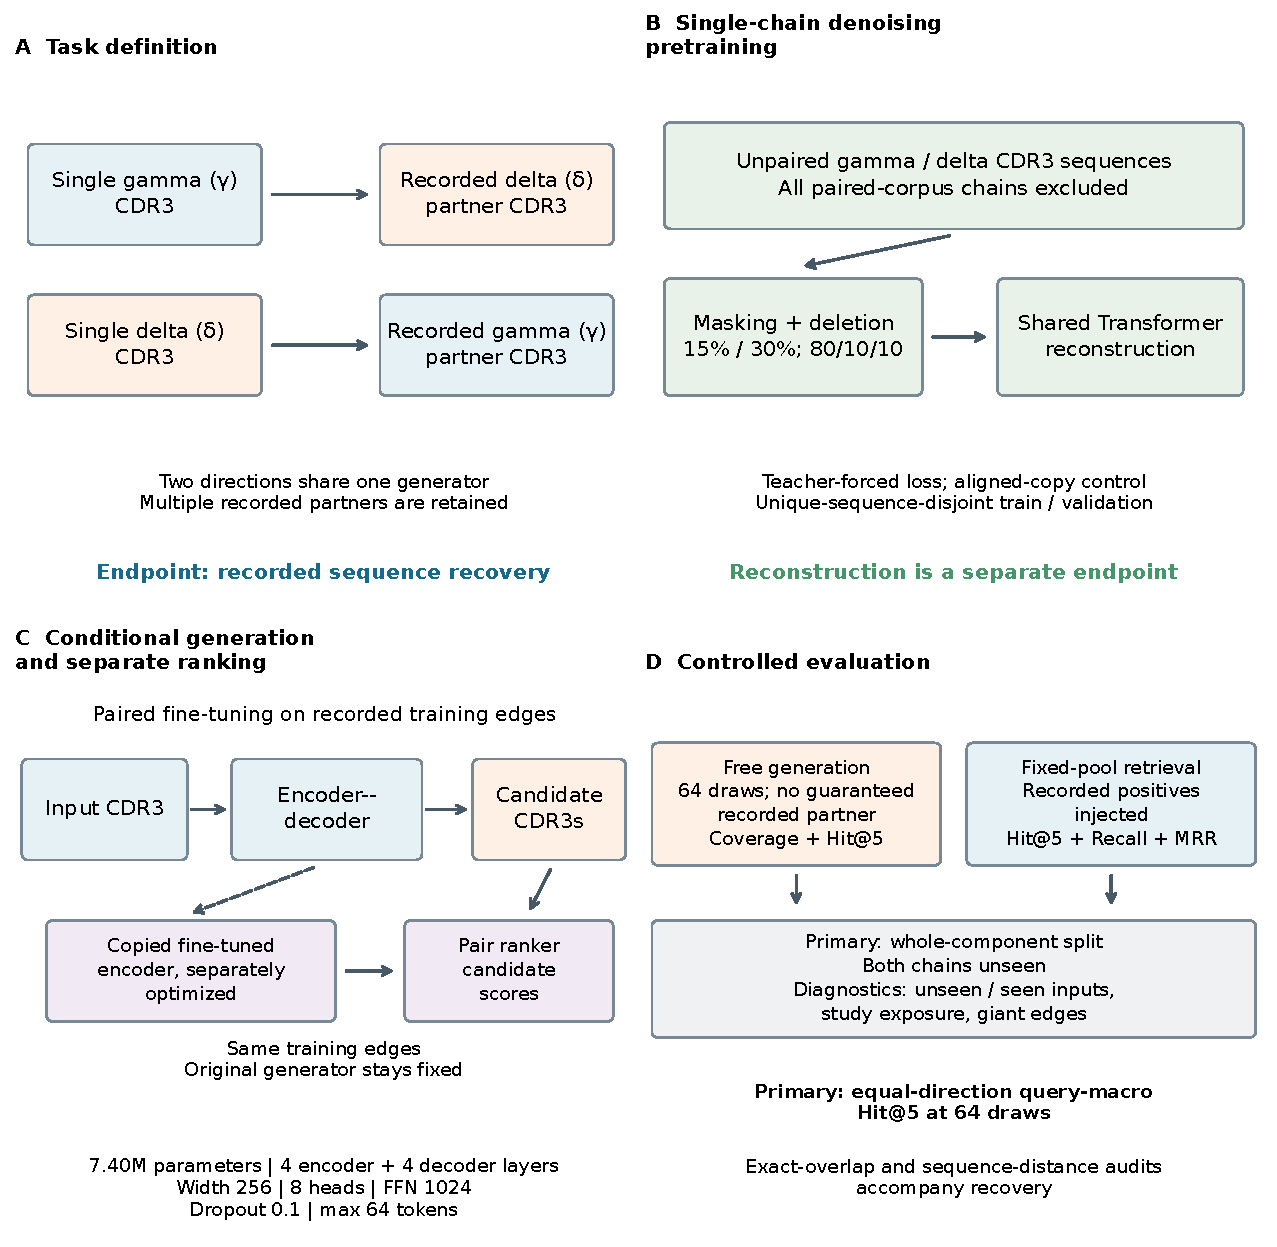
\includegraphics[width=\linewidth]{results/bmc/figures/figure_1_workflow.pdf}
\caption{Overview of the single-CDR3 partner-recovery benchmark and model workflow. A: each task maps one gamma or delta CDR3 to recorded partner CDR3s. B: denoising pretraining excludes all paired-corpus chains. C: conditional generation and separately trained ranking share training-edge and encoder provenance. The ranker optimizes its copied encoder; the original generator remains fixed. D: free generation and truth-containing retrieval are different endpoints. The primary endpoint is equal-direction mean query-macro Hit@5 at 64 draws under component-disjoint splitting; other exposure protocols are diagnostics.}
\label{fig:workflow}
\end{figure}

\begin{figure}[htbp]
\centering
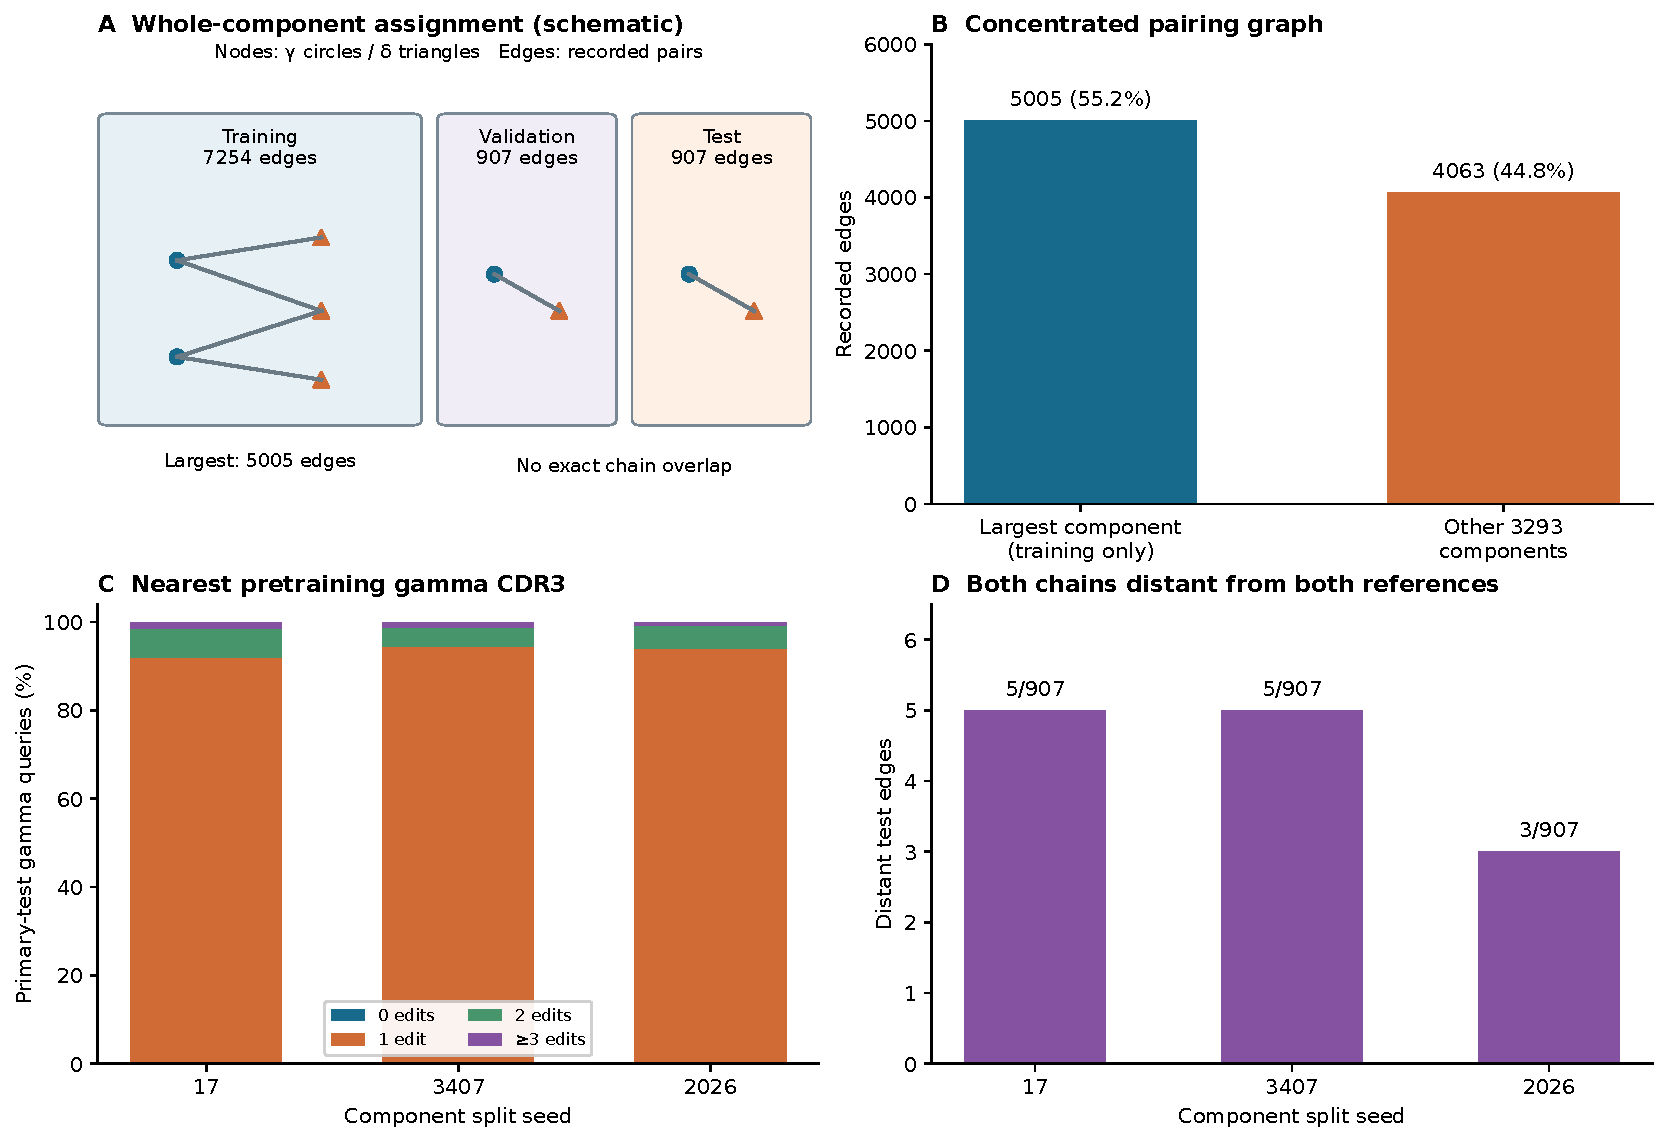
\includegraphics[width=\linewidth]{results/bmc/figures/figure_2_data.pdf}
\caption{Pairing-graph concentration and sequence exposure. A: schematic component assignment, with all 5005 edges of the largest component retained in training. Nodes are unique gamma/delta CDR3s and edges are publicly recorded pairs. Primary partitions have no exact chain overlap. B: observed component concentration. C: minimum full-CDR3 Levenshtein distance to the pretraining pool. D: a distant edge requires both chains to be at least three edits from both supervised and pretraining references. The 5/5/3 distant-edge counts are too small for stable inferential transfer claims. This figure describes dataset exposure, not a recovery endpoint.}
\label{fig:data}
\end{figure}

\begin{figure}[htbp]
\centering
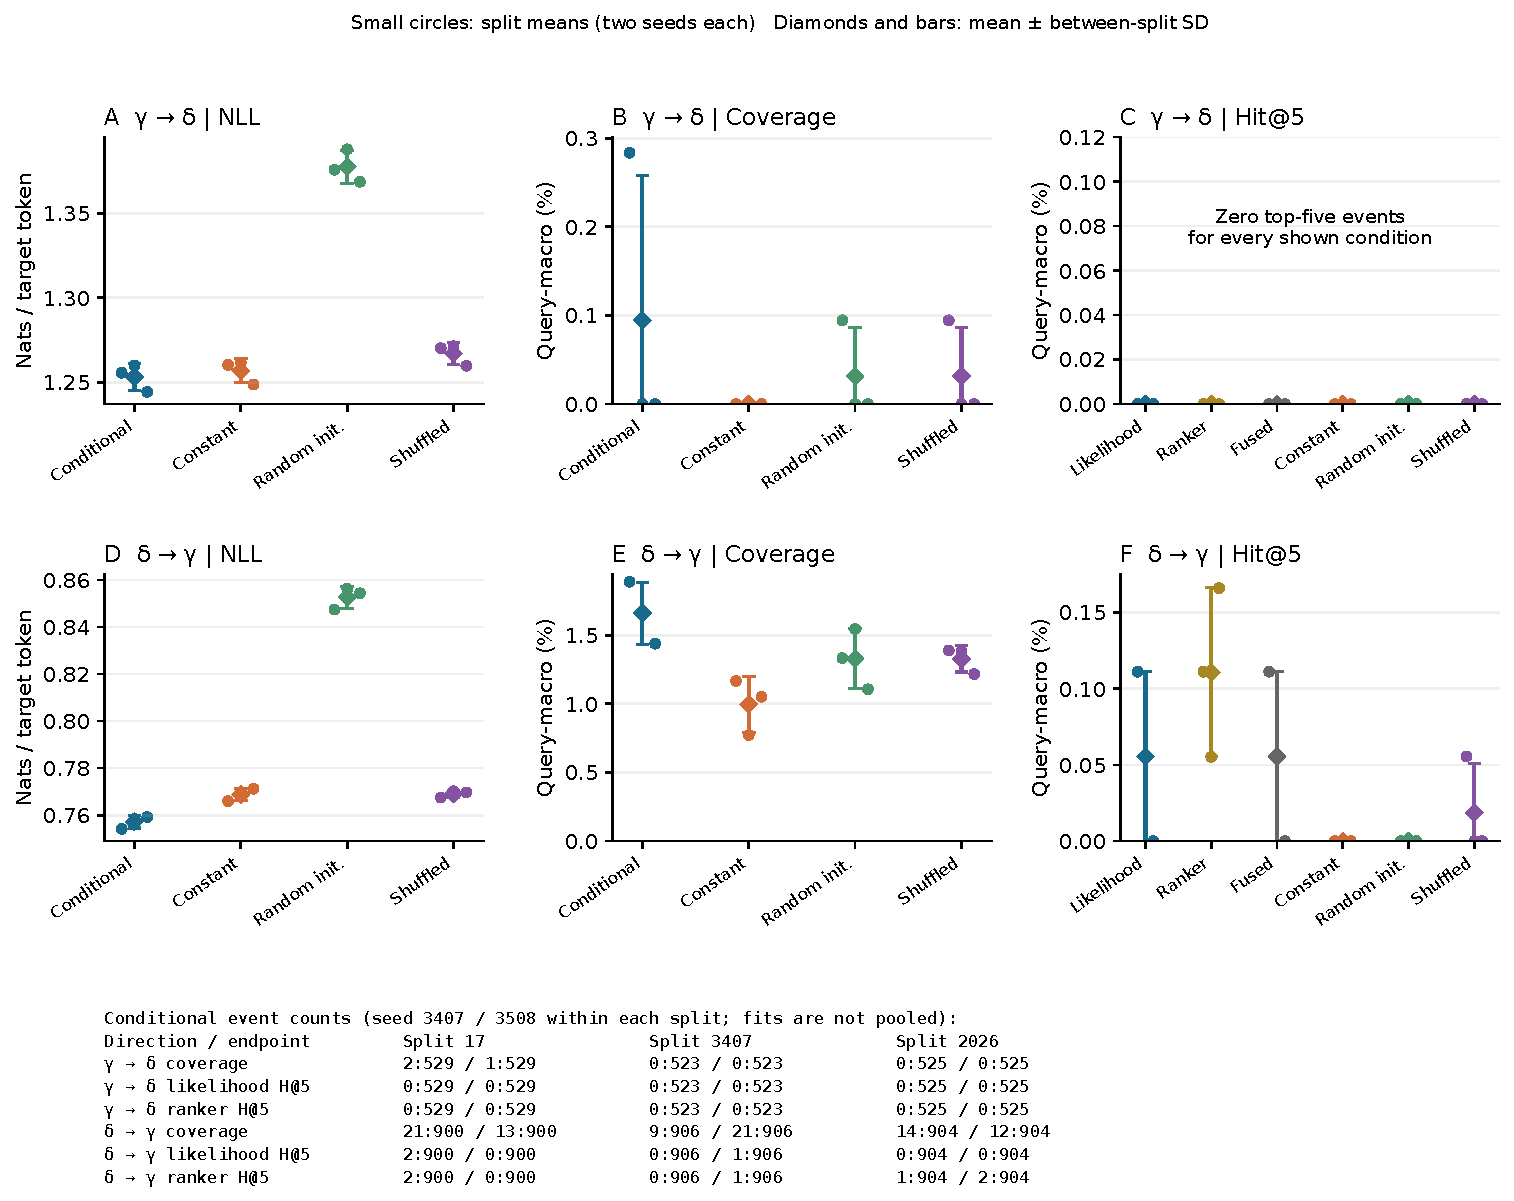
\includegraphics[width=\linewidth]{results/bmc/figures/figure_3_primary.pdf}
\caption{Sparse free recorded-partner recovery at 64 draws. No recorded positive is injected into free candidates; training targets are allowed. Conditional, constant-source, random-initialization and shuffled-input conditions share the evaluation rule. Points are three split means after averaging two model seeds; diamonds and ranges are their mean and descriptive SD, not subject-level confidence intervals. Likelihood, ranker and fused scores order identical conditional candidates. The graphic gives conditional events:query counts for each fitted model; all conditions are tabulated in Additional file 4. Zero events are retained. A lower NLL does not imply reliable candidate availability or top-five recovery.}
\label{fig:primary}
\end{figure}

\begin{figure}[htbp]
\centering
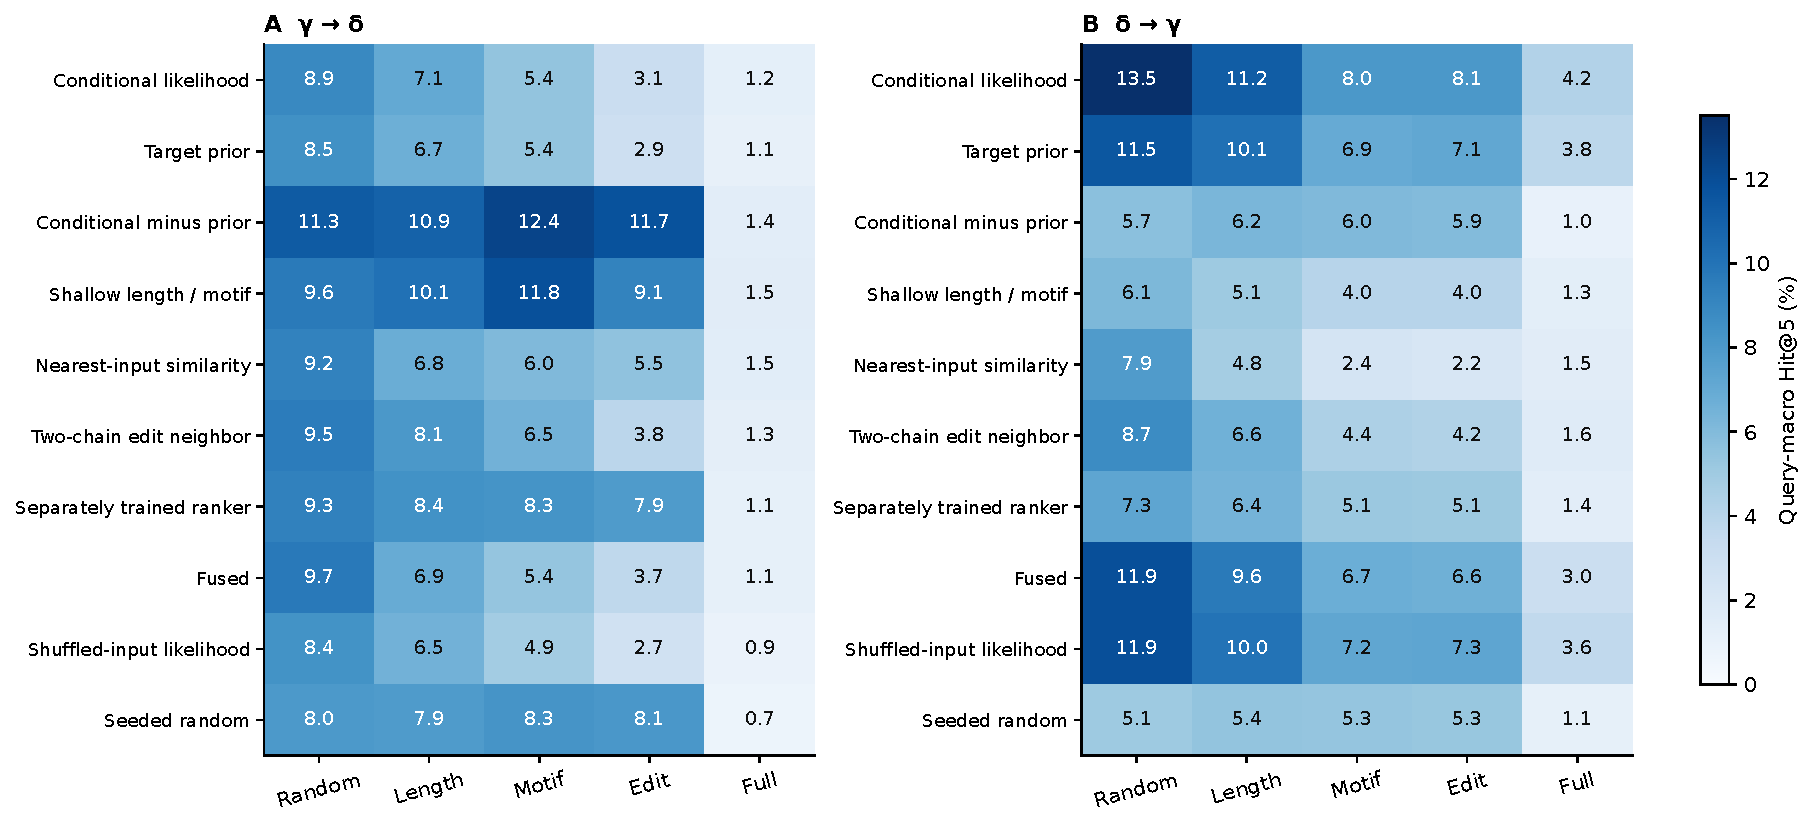
\includegraphics[width=\linewidth]{results/bmc/figures/figure_4_retrieval.pdf}
\caption{Ranking within truth-containing fixed candidate pools. Fixed pools contain recorded positives by construction. Random, length, motif and edit pools add up to 100 unrecorded distractors; Full uses the complete role-specific target universe. Values average seeds within split and then the three primary splits equally. Deterministic methods have one value per split. Nearest-input similarity scores candidates by target distance to partners of the single nearest training input; direct partner transfer is reported separately. No scorer dominates all pools and directions. These retrieval outcomes cannot be equated with free-generation recovery or biological specificity.}
\label{fig:retrieval}
\end{figure}

\begin{figure}[htbp]
\centering
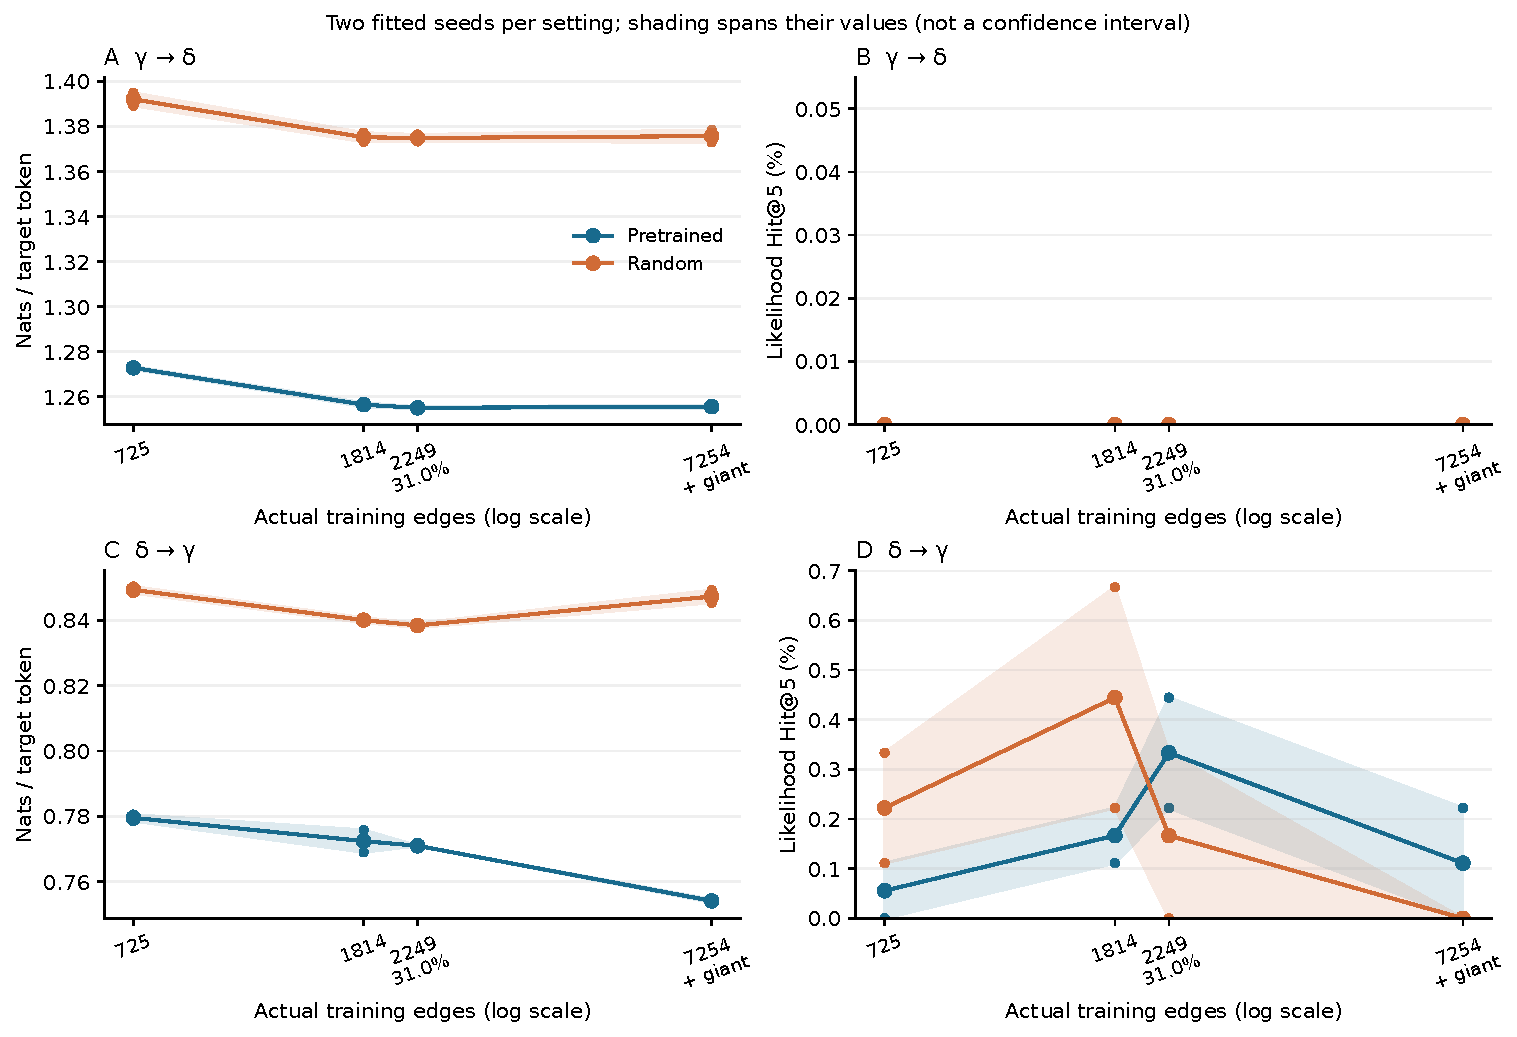
\includegraphics[width=\linewidth]{results/bmc/figures/figure_5_efficiency.pdf}
\caption{Likelihood and recovery across nested complete-component training subsets. The actual subsets contain 725/1814/2249/7254 edges. The nominal 50\% subset contains only 31.0\% of training edges. All smaller subsets contain singleton components; the giant component enters only at full data, so composition and size change together. Lines average two model seeds and shading spans their fitted estimates; it is not a confidence interval. Lower NLL does not provide a consistent small-data free-recovery advantage.}
\label{fig:efficiency}
\end{figure}

\begin{figure}[htbp]
\centering
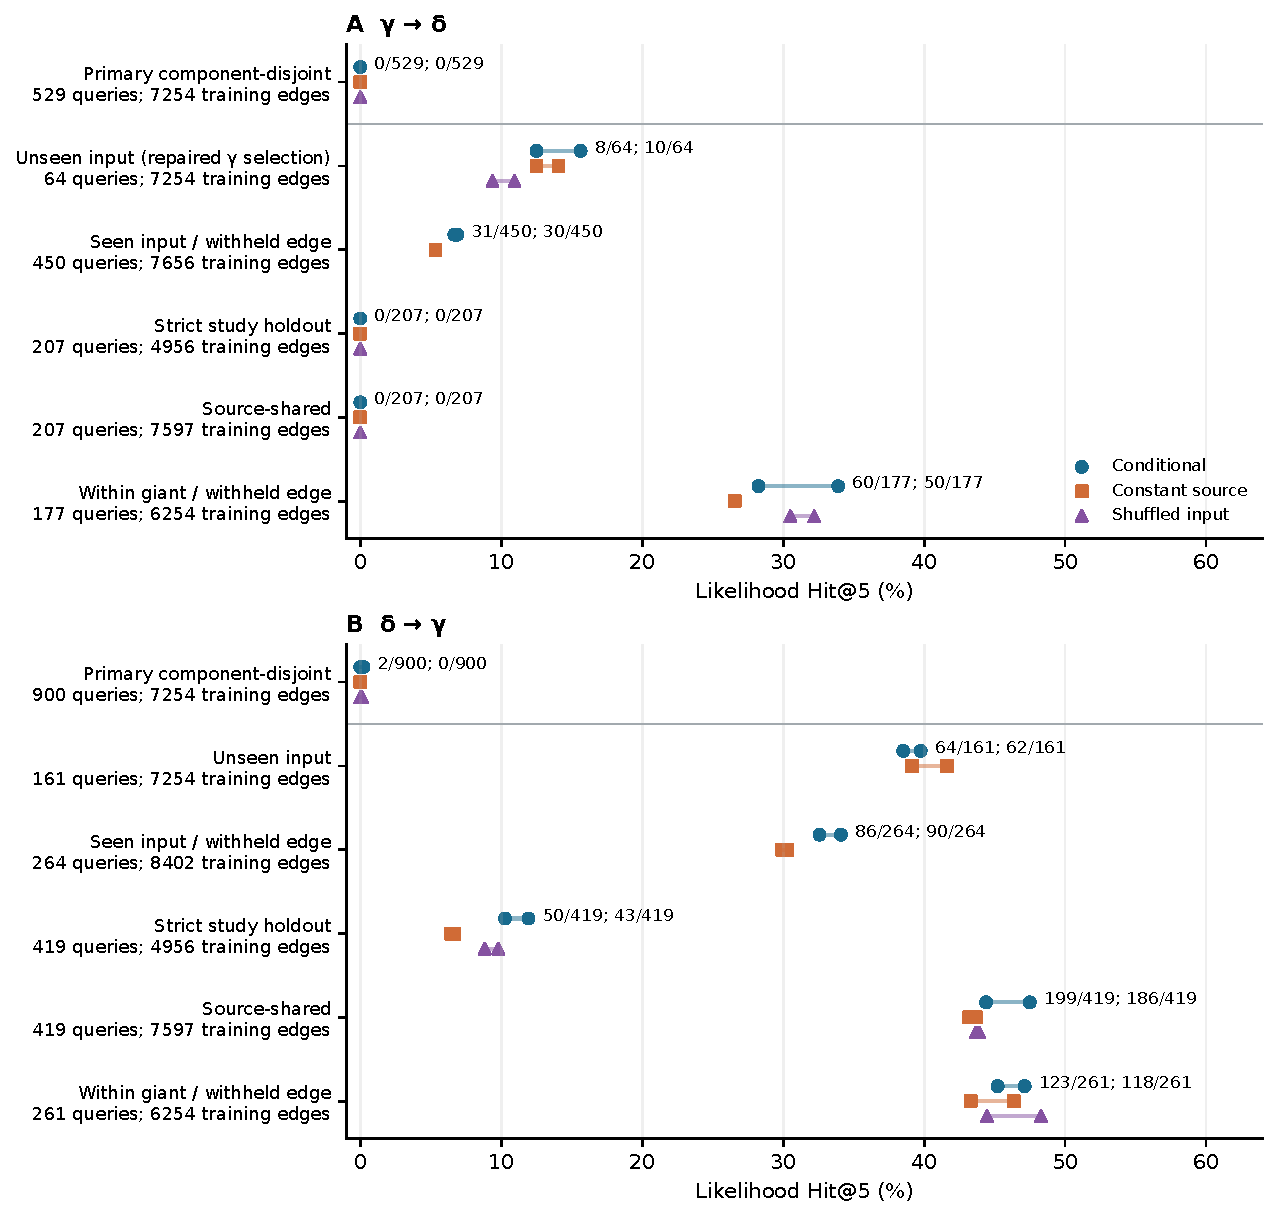
\includegraphics[width=\linewidth]{results/bmc/figures/figure_6_protocols.pdf}
\caption{Recovery across distinct exposure populations. Each point is one model seed at 64 free draws; labels give conditional events/queries in seed order 3407;3508. The first row is the primary split-17 reference; all other rows are diagnostic populations with different training composition. Original unseen-gamma selection used a single query and had degenerate MRR; the plotted revision refits use 31 selection queries, leaving train/test membership unchanged. Unseen-input tasks permit target exposure; seen-input and within-giant tasks retain supervised input exposure, with both endpoints exposed in the latter. Missing shuffled points in original directional tasks mean not evaluated. Strict study holdout excludes held-study chains; source-shared retains common chains. Neither is donor-independent external validation. All within-giant edges arise from one original component; no inferential component interval is asserted.}
\label{fig:protocols}
\end{figure}

\begin{figure}[htbp]
\centering
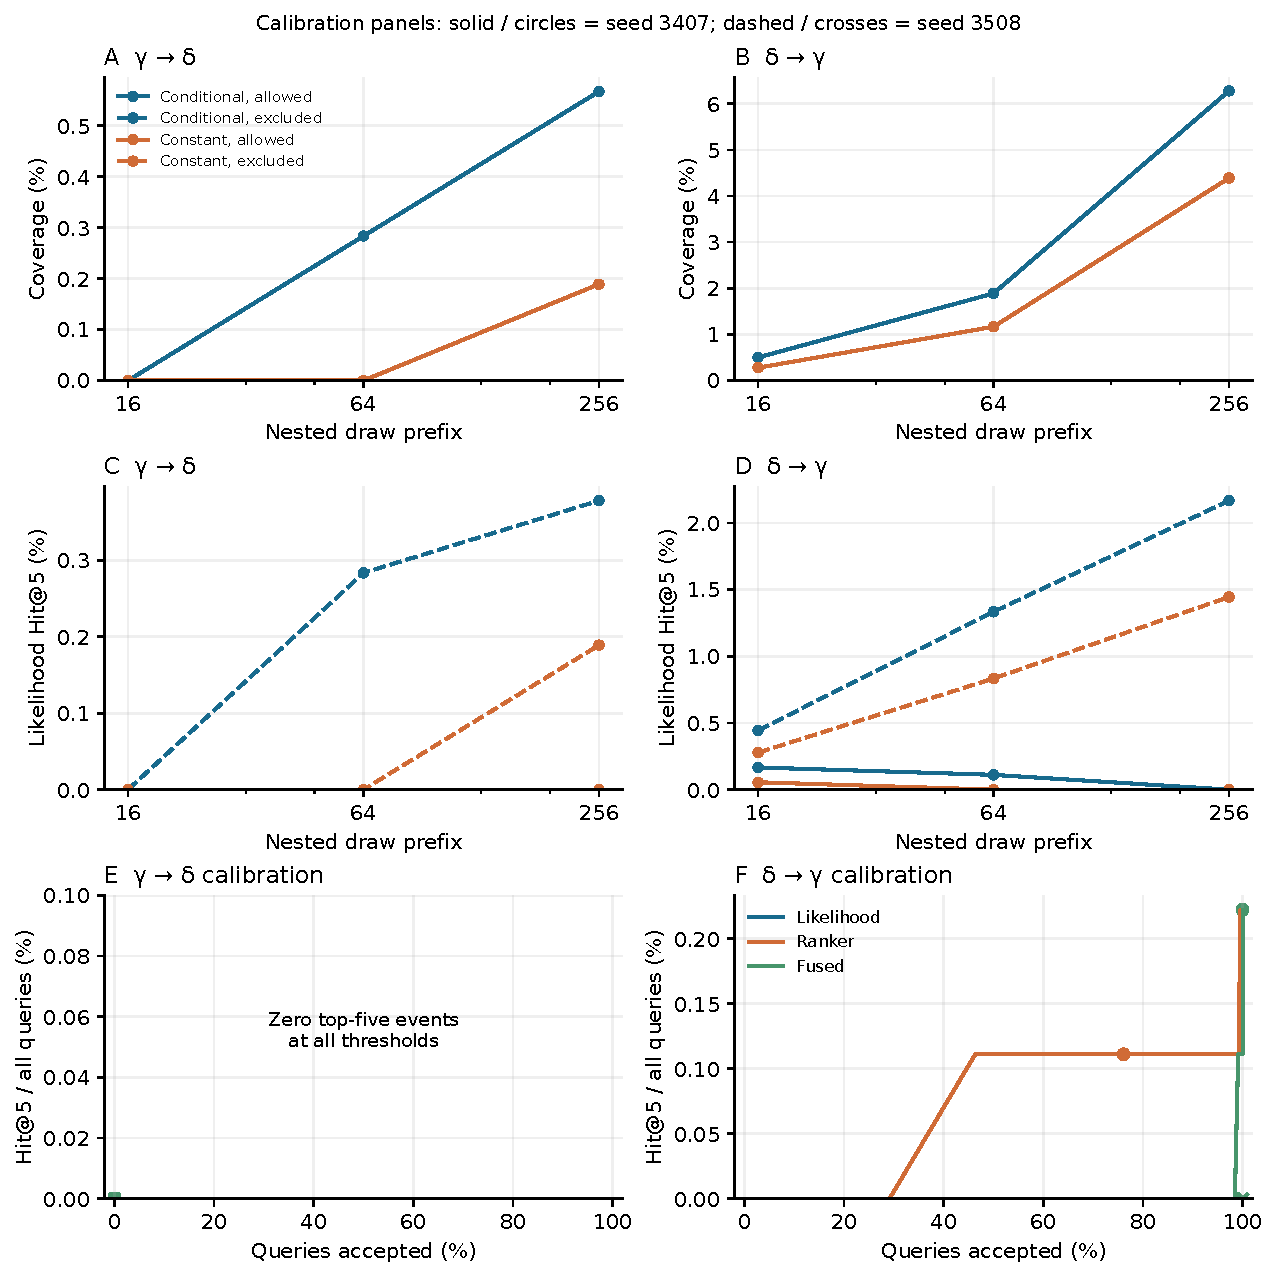
\includegraphics[width=\linewidth]{results/bmc/figures/figure_7_budget.pdf}
\caption{Sampling budgets and exploratory calibration. The 16/64/256 budgets are prefixes of the same saved draws on split 17. Left and middle panels separate candidate coverage from likelihood Hit@5, with exact training targets allowed (solid) or excluded (dashed); lines average two seeds. Coverage is unchanged by target exclusion in the chain-disjoint primary test. Right panels are exploratory calibration-quantile operating curves; solid/dashed lines identify seeds and markers identify independently calibrated thresholds. All test queries remain in recovery denominators. More draws can increase coverage without improving top-five ordering. No threshold is a validated biological selector.}
\label{fig:budget}
\end{figure}
% END BMC FIGURES
\end{document}
